\section{Теоретическая информация}
\subsection{Метод конфигурационного взаимодействия}
Метод конфигурационного взаимодействия (КВ или CI -- configuration interaction) позволяет учесть корреляционные эффекты в молекулярной системе. В данном методе волновая функция раскладывается в ряд по детерминантам Слейтера $\Psi_k$, каждый их которых описывает систему в некотором электронном состоянии. Одно из таких состояний $\Psi_0$ является основным. Остальные состояния описываются электронными конфигурациями, в которых последовательно учтены возможные переходы электронов с занятых МО на различные незанятые (виртуальные) орбитали. Такие состояния также называют возбужденными. Эти состояния классифицируют по числу МО, замещенных виртуальными (одно-, дву-, трех-, \ldots, N-кратно замещенные детерминанты). 

Полная волновая КВ-функция, учитывающая все возможные электронные конфигурации, имеет вид
\mequation{
    \Psi_{CI} = a_0\Psi_0 + \sum\limits_{k=1}^{\infty}a_k\Psi_k
}
и находится с помощью вариационного принципа (аналогично тому, как сделано в методе Ритца). При этом спин-орбитали в каждом слейтеровском детерминанте $\Psi_k$ остается неизменными в течение всего расчета\footnote{Однако в более продвинутом методе MCSCF (Multi-Configurational Self-Consistent Field) оптимизируются не только коэффициенты, но и сами спин-орбитали.}.

\begin{figure}[H]
\centering
\captionsetup{justification=centering}
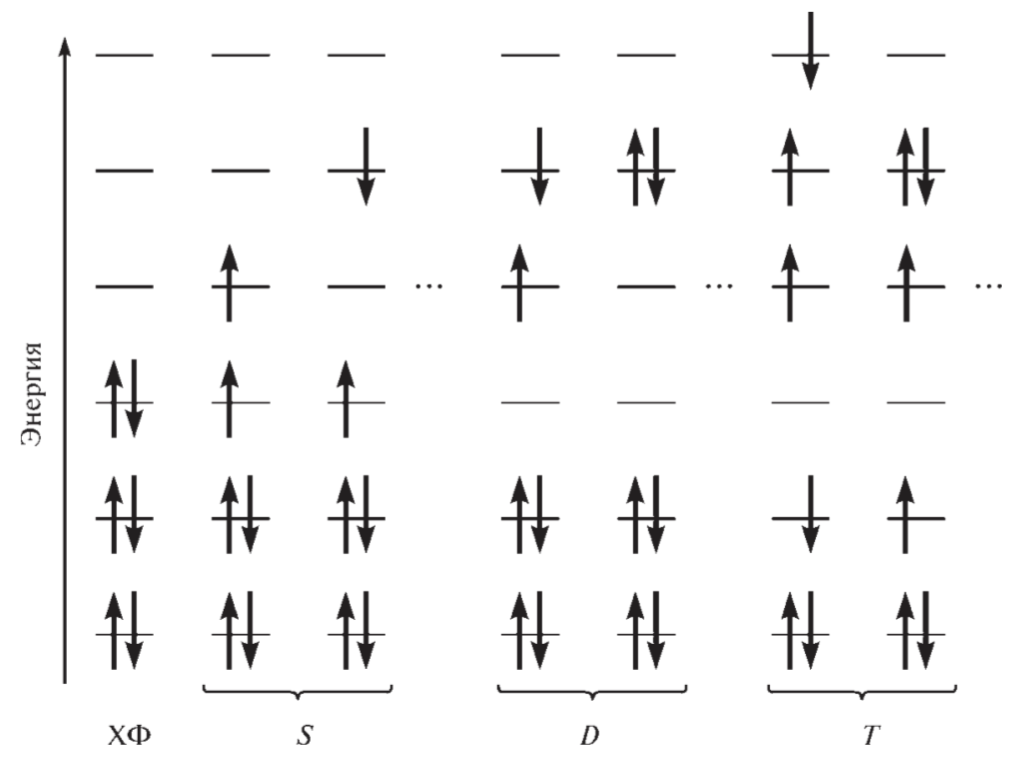
\includegraphics[scale=0.5]{fig/2.png}
\caption{Схема, иллюстрирующая формирование замещенных электронных конфигураций путем перемещения в детерминантах Слейтера электронов с МО, занятых в основном состоянии, на виртуальные МО. ХФ обозначает электронную конфигурацию основного состояния ( полученного методом Хартри—Фока). Буквами S, D и T обозначены одно-, дву- и трехкратно замещенные конфигурации соответственно}
\end{figure}

Действуя аналогично тому, как сделано в методе Ритца, для коэффициентов $a_k$ получим следующую систему линейных уравнений
\mequation{
    \sum\limits_{k=0}^{n-1}a_{k}\left(H_{k', k} - \epsilon S_{k', k} \right) = 0, k' = 0, 1 \ldots n - 1
}
где $n$ -- число учитываемых электронных состояний, $\epsilon$ -- неопределенный множитель, $H_{k', k} = \int\Psi_{k'}^{\ast}H\Psi_{k}dV$ -- матричные элемент оператора Гамильтона, $S_{k', k} = \int\Psi_{k'}^{\ast}\Psi_{k}dV$ -- интеграл перекрывания электронных состояний.

У данной системы имеется нетривиальное решение, когда детерминант равен нулю
\mequation{
    det(H_{k', k} - \epsilon S_{k', k}) = 0
}

Данная система является уравнением степени $n$ относительно величины $\epsilon$ и имеет $n$ корней. Выбирая различные решения этого уравнения и подставляя их в систему выше, получим $n$ наборов коэффициентов и, соответственно, $n$ различных электронных состояний. Физический смысл значения $\epsilon$, соответсвующее конкретному набору коэффициентов, -- энергия электронного состояния. Минимальное значение $\epsilon$ соответсвует энергии основного состояния, следующее по величине -- первого возбужденного состояния и т.д.

Хочется отметить, что название “метод конфигурационного взаимодействия” не совсем удачное. В данном методе не подразумевается никакое взаимодействие электронный состояний. Основная идея введения новых электронных состояний -- увеличить разложения волновой функции, тем самым приблизив полученную волновую функцию к точной.